\begin{frame}{破裂高度帯は春と秋に風向が読めない}{結果：北海道}
  \begin{columns}[T]
    \begin{column}{0.56\textwidth}
      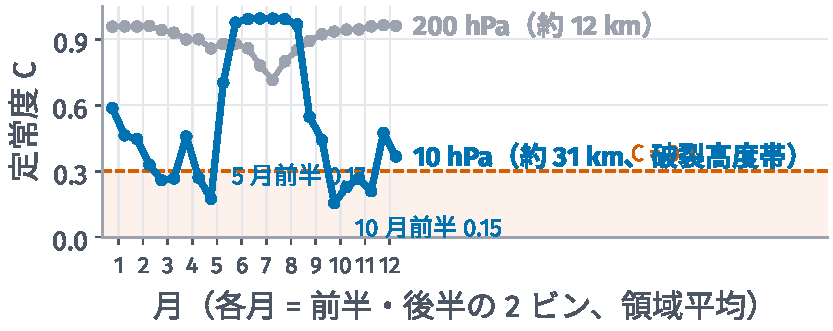
\includegraphics[width=\linewidth,height=118pt,keepaspectratio]{S_constancy_10hpa.pdf}
      \vskip 0.5mm
      \sub{夏 0.99、春 0.35、秋 0.31。東西逆転の時期は\\\kw{西風の日}と\kw{東風の日}が混ざり、打ち消し合う。}
    \end{column}
    \begin{column}{0.42\textwidth}
      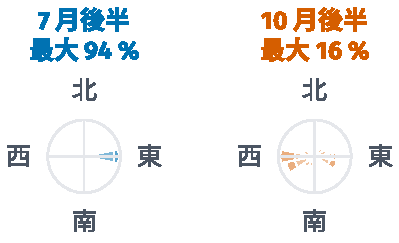
\includegraphics[width=\linewidth,height=96pt,keepaspectratio]{S_roses_10hpa.pdf}
      \vskip 0.5mm
      \sub{\warn{データが無いのではない}。\\平均風向に意味がない。}
    \end{column}
  \end{columns}
  \srcline{10 hPa（約 31 km）。定常度は領域平均、風配図は 1 格子点（半径は図ごと）}
\end{frame}
